\documentclass[11pt]{article}
\usepackage{../EllioStyle}

\title{Homework 2}
\author{Elliott Pryor}
\date{11 Feb 2021}

\rhead{Homework 2}
\lhead{Elliott Pryor}

\graphicspath{{./}{images/}}


\makeatletter
\def\mathcolor#1#{\@mathcolor{#1}}
\def\@mathcolor#1#2#3{%
  \protect\leavevmode
  \begingroup
    \color#1{#2}#3%
  \endgroup
}
\makeatother


\algdef{SE}[DOWHILE]{Do}{doWhile}{\algorithmicdo}[1]{\algorithmicwhile\ #1}

\begin{document}
\maketitle

\problem{1}

Assume you are given a planar subdivision with $n$ faces in a DCEL. (You may
assume that the planar subdivision does not contain any holes, i.e., there are
no nested faces.) Give pseudo-code for an algorithms that given a vertex $v$ of
the DCEL, outputs all neighbors of $v$.

\hrule

\begin{algorithm}
    \caption{Find Neighbors}
    \label{alg:neighbors}
    \begin{algorithmic}[1]
    \Function{Neighbors}{$v$}
        \State $start \gets v.incident\_edge$
        \State $e \gets start$
        \Do
            \State $twin \gets e.twin$
            \State add $twin.origin$ to neighbors
            \State $e \gets twin.next$
        \doWhile{$e \neq start$}
        \State \textbf{return} neighbors
    \EndFunction
    \end{algorithmic}
\end{algorithm}


\begin{figure}[h]
    \centering
    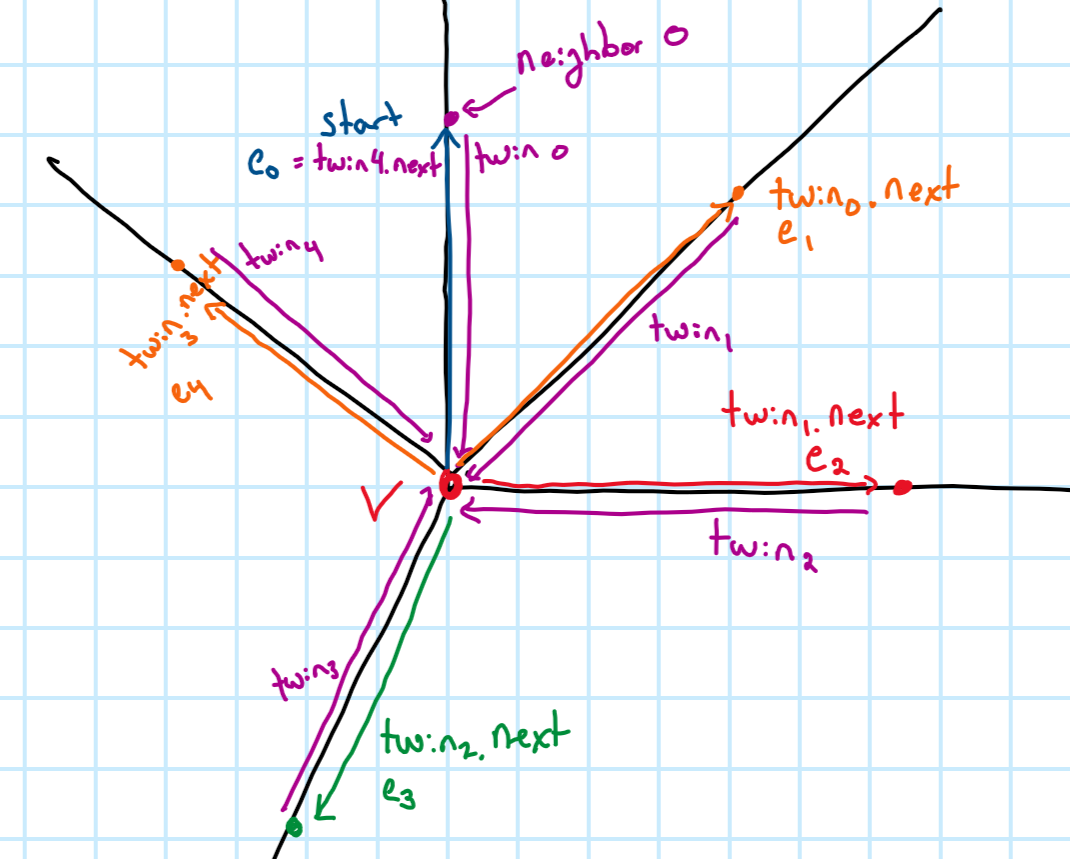
\includegraphics[width = 0.65\textwidth]{prob1}
    \caption{Problem 1: Visual demonstration of algorithm}
\end{figure}

\textbf{Correctness:} The algorithm starts with the incident edge to vertex $v$. 
Since we only store the origin of each edge, the origin of the twin is the same as the destination.
This is a neighbor of $v$ since it is 1 edge away. 
Then, we observe that if $e$ is incident on the left face, then $e.twin$ is incident on the right face.

We also know that the destination of $e.twin$ is $v$. So $e.twin.next$ must be another neighbor of $v$.
This is the next neighbor clockwise around $v$. Suppose we skipped a neighbor then there must be a face in between.
But then twin would have to be incident on the middle face (one in between), so a contradiction and we find the next node clockwise.

So we always find the next neighbor clockwise around $v$, until we reach the start when we terminate.

\textbf{Running Time:} We cover each face that $v$ is incident upon once. Therefore our time is $O(n)$




\problem{2}

Assume you are given a planar subdivision of $O(n)$ size in a DCEL. (You may
assume that the planar subdivision does not contain any holes, i.e., there are
no nested faces.) Describe an algorithm that for a given point $p$ in the plane
finds the face in the subdivision that contains it. Your algorithm should run in
$O(n)$ time. You do not have to write pseudo-code, but please make clear what
DCEL operations you are using. Also please make sure the analysis is detailed
enough to justify the $O(n)$ runtime clearly.

\hrule



\begin{algorithm}
    \caption{Find what face Point is in}
    \label{alg:point}
    \begin{algorithmic}[1]
    \Function{FindFace}{$p$}
        \For{face $\in$ Faces}
            \State $start \gets face.incident\_edge$
            \State $e \gets start$
            \State $intersections \gets 0$
            \Do
                \State $origin \gets e.origin$, $destination \gets e.twin.origin$
                \State $l \gets$ line through edge $e$
                \State $i \gets $ point where $l(x) = p_y$ \textcolor{red}{point where line interesects y level of p}
                \If{$i.x \geq p.x$ and $i.x \in [origin.x, destination.x]$}
                    \State \textcolor{red}{Found an intersection!}
                    \State increment $intersections$
                \EndIf
                \State $e \gets e.next$
            \doWhile{$e \neq start$}
            \If {$intersections \mod  2 = 1$}
                \State \textbf{return} face
            \EndIf
        \EndFor
    \EndFunction
    \end{algorithmic}
\end{algorithm}




\problem{3}

Assume you are given a collection of $n$ circles $\{C_1 , \ldots , C_n \}$ in
$\reals^2$, where circle $C_i$ is presented as its center point $q_i = (x_i, y_i)$
and radius $r_i > 0$. Present an $O(n \log n)$ time algorithm that determines
whether any two circles intersect. Note that one circle may be nested within
another without intersecting (see Figure 1). Your algorithm should either output
that there is no intersection, or that there is at least one intersection, and
if so it will output the indices of $i$ and $j$ of two circles $C_i$ and $C_j$
that intersect. Irrespective of the number of intersecting pairs, it need only
output one intersecting pair.

\begin{figure}[h]
    \centering
    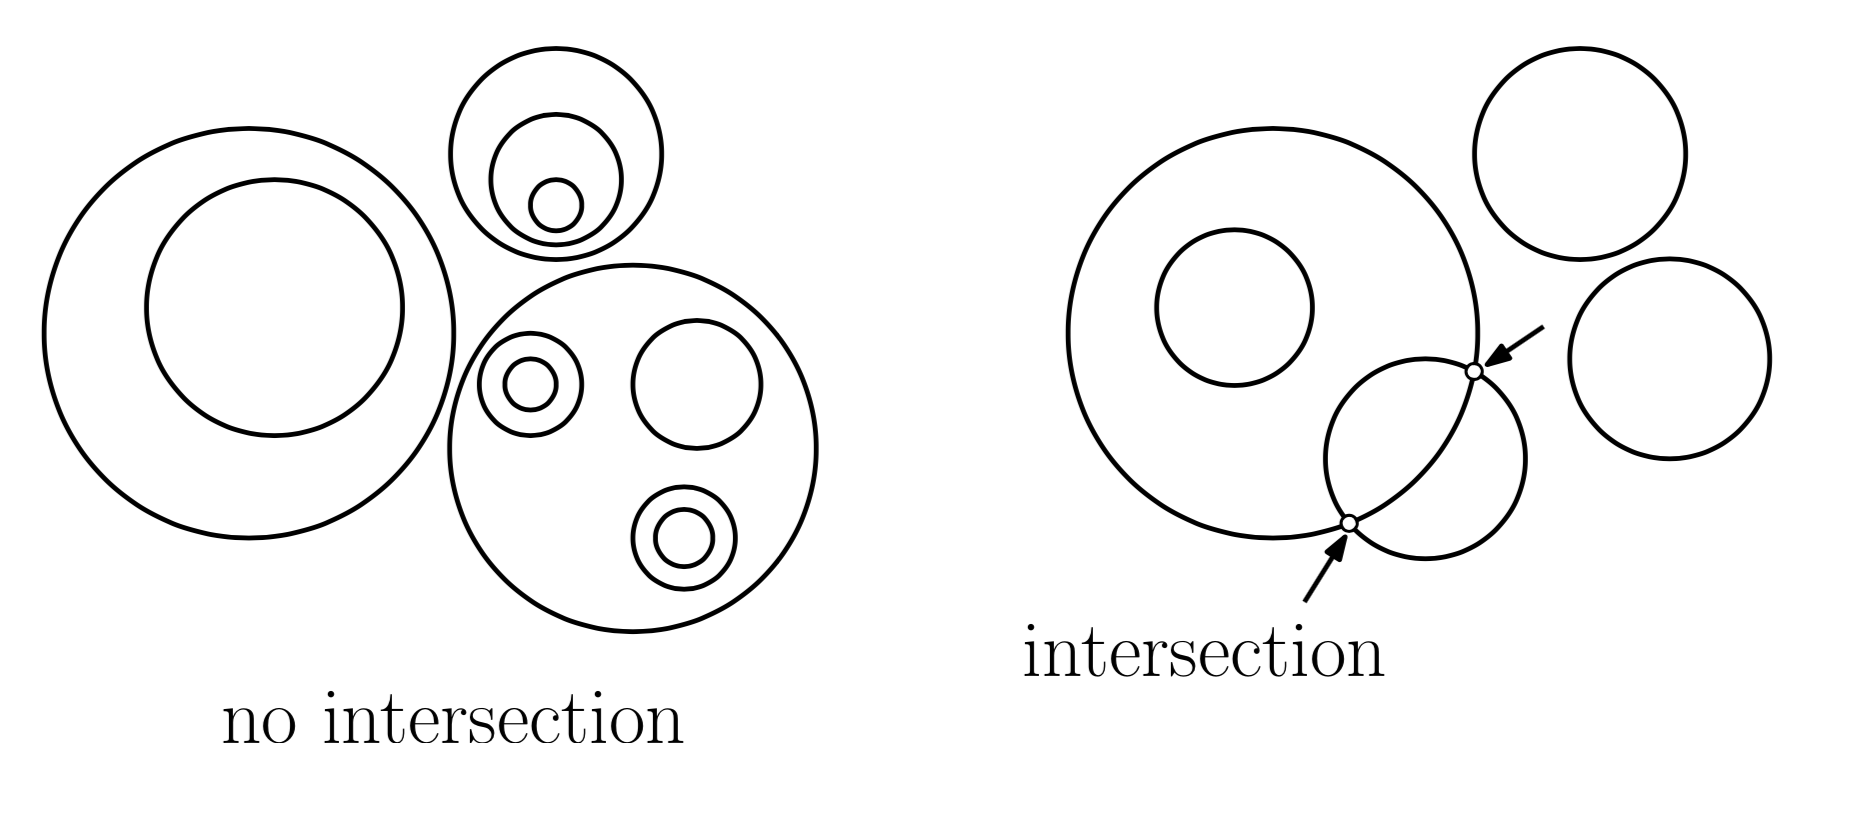
\includegraphics[width=0.75\textwidth]{intersection}
    \caption{Problem 3: Intersection}
\end{figure}

Hint: Use plane-sweep. Explain clearly (1) what the sweep-line status stores and
what data structure is used to store this information and (2) what future events
are stored and what data structure is used. You may assume that you have access
to whatever primitive operations that you need in constant time. For example, if
you want to determine (a) whether two circles intersect, (b) the coordinates of
an intersection, (c) the intersection of a line with a circle, (d) whether a
point is contained within a circle's interior, etc., you may simply assume the
existence of a function that runs in $O(1)$ time. As always, you may make
whatever general-position assumptions you like.

\hrule


So the strategy is to split the circles into two semi circles and treat them individually.
This runs essentially the same as the original line-sweep algorithm for line segments.
The intersection computation is harder since they are not lines, but it can be done in constant time since we have formulas for semi-circles.

\begin{enumerate}[(1)]
    \item The sweepline status stores the semi-circular curves.
        These are stored in a dictionary (balanced tree) and are sorted by the y coordinate.
    \item Our events are the endpoints (left and right) of every circle. 
    Then, at runtime, when a new event occurs curve intersection is computed between adjacent 
    two semi-circles. If they intersect, a new event is placed at the intersection location. 
    These events are stored in a priority queue. 
\end{enumerate}





\problem{4}

I have had a few people ask about drawings and making figures.  One tool that I
like to use is Ipe (written by Otfried Cheong).  Ipe allows you to draw content
on layers and show and hide the different layers.  Layers are very helpful if,
for example you want to draw a point set and then show how some data structures
in an algorithm change as you sweep across the point set.
Other vector graphics tools such asIllustrator and Inkscape are also quite good.

Setup Ipe \url{http://ipe.otfried.org/}, Illustrator, or Inkscape
(or another vector graphics tool)
to create 3 images of the state of the sweep line algorithm
described in problem 3.

\hrule




\end{document}